\chapter{Results}

\section{Intensity of single source - Diffraction}

Using python, I plotted distance vs. intensity for a single source. The relevant python code can be found in appendix \ref{code:single}.

\begin{figure}[!h]
\centering	
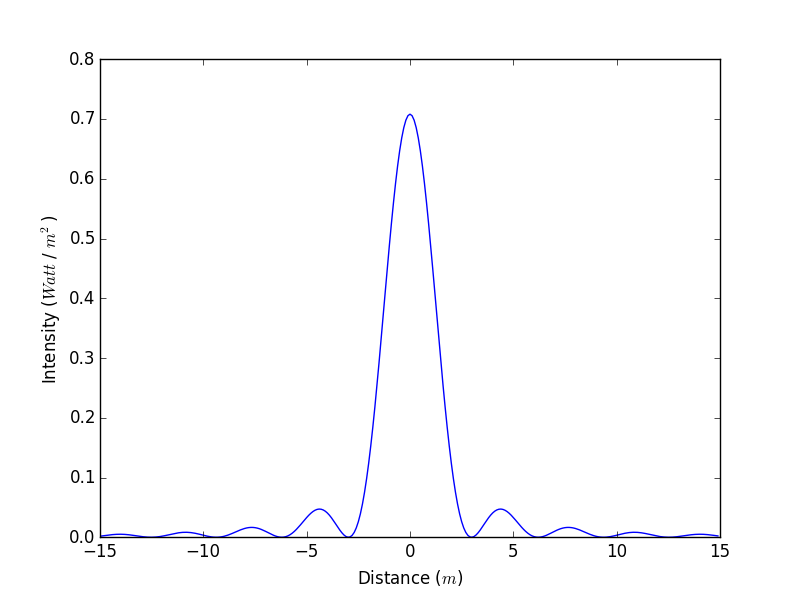
\includegraphics[scale=0.45]{figure_1.png}
\caption{Intensity profile of single antenna}
\end{figure}

As it should be, Intensity decreases by increasing the distance. Where at the position where source is placed we have high intensity peak.

\section{Intensity of linear array of 4 antennae}

Plot between distance and intensity, for four antenna sources arrange in a linear array and by managing phase between them, we get interference pattern. The relevant code can be found in appendix \ref{code:four}.

\begin{figure}[!h]
	\centering	
    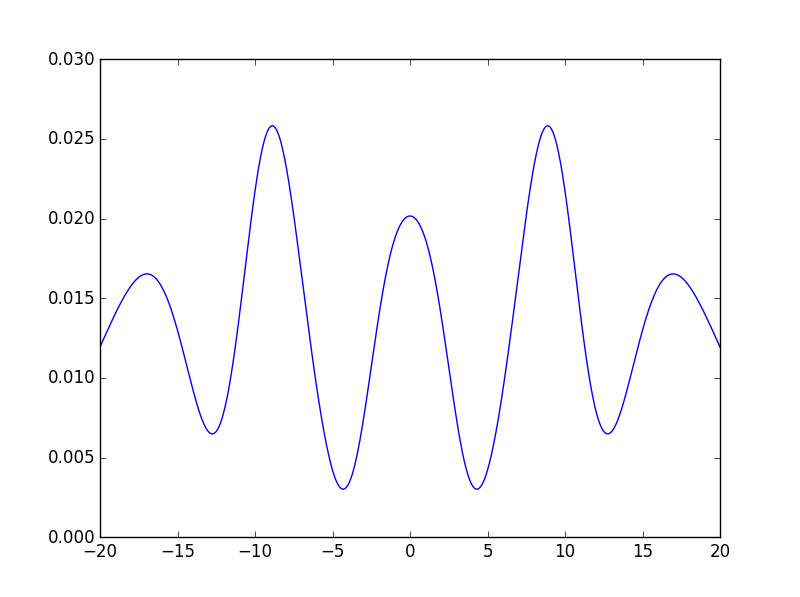
\includegraphics[scale=0.45]{figure_2.png}
	\caption{Intensity profile of linear array of 4 antennae}
\end{figure}

\subsection{Introducing Phase}

Fig. (1.2) shows a plot between distance and intensity, for four antenna sources arrange in a linear array. Now, by introducing and managing phase among them we can steer the beam as:

\begin{figure}[!h]
	\centering	
	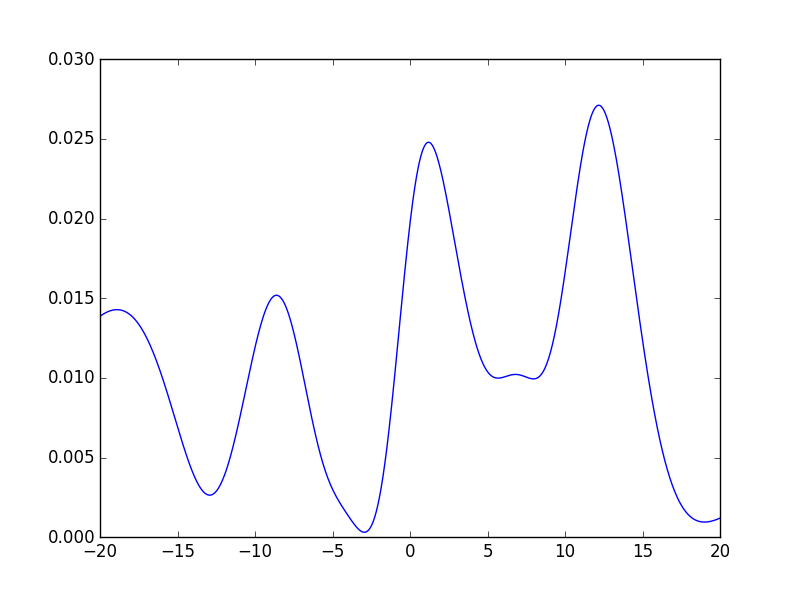
\includegraphics[scale=0.45]{figure_3.png}
	\caption{Intensity profile of linear array of 4 antennae}
\end{figure}

\begin{figure}[!h]
	\centering	
	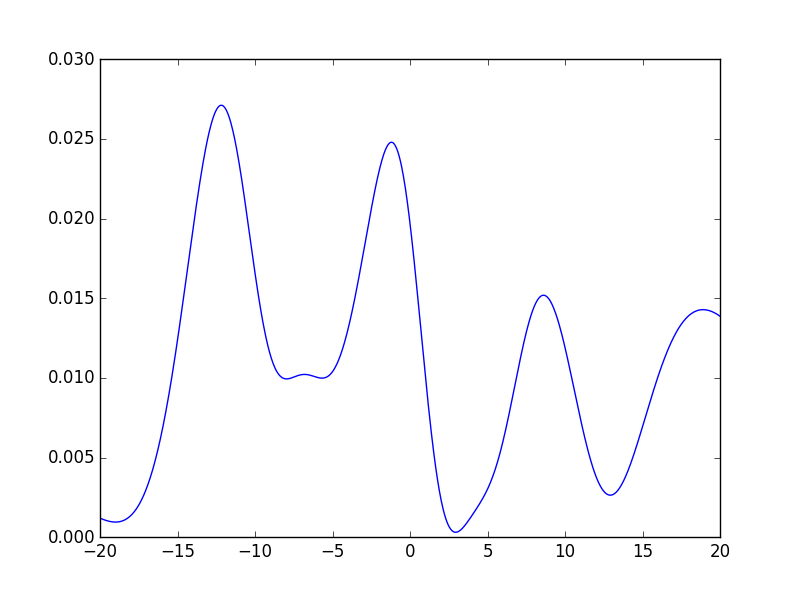
\includegraphics[scale=0.45]{figure_4.png}
	\caption{Intensity profile of linear array of 4 antennae}
\end{figure}
